\documentclass[a4paper, 11pt]{article}
\usepackage{comment} 
\usepackage{fullpage} 
\usepackage[spanish]{babel} 
\selectlanguage{spanish}
\usepackage[utf8]{inputenc}
\usepackage{float} 
\usepackage{graphicx}
\usepackage{ marvosym }
\usepackage{amsthm}
\usepackage{amsmath}
\usepackage[sort&compress, numbers]{natbib}
\usepackage{amssymb}
\usepackage{hyperref}
\hypersetup{colorlinks=True, citecolor=blue}


\begin{document}
\begin{center}
\LARGE \bf Pr\'actica 3\\ Teoría de colas 
\end{center}

\vspace{1cm} 
\noindent\textbf {Edson Edgardo Samaniego Pantoja} \hfill \textbf{Materia:} Simulación computacional 
\hfill \\
\textbf{Fecha} \today  
\vspace{1cm} 

\section{Introducción}
La teoría de colas es el estudio matemático de las colas o líneas de espera en un sistema, esta teoría se presenta cuando los \textit{clientes} llegan a un \textit{lugar} demandando un servicio a un \textit{servidor}, el cual tiene una cierta capacidad de atención. Si dicho \textit{servidor} no esta disponible o tiene atraso se generan líneas de espera. Estudia factores como el tiempo de espera medio en las colas o la capacidad de trabajo del sistema sin que llegue a colapsar.

\section{Objetivo}
El objetivo de esta práctica es examinar las diferencias en los tiempos de ejecución de diferentes ordenamientos de conjuntos de datos cuando se varían el número de núcleos que procesan estas tareas. Utilizando como datos de entrada un vector que contiene números primos grandes que se obtuvieron de la pagina PrimePages \cite{primos} y no-primos que se extraen entre cada salto de números primos. Como condición se utilizan números de nueve dígitos y se aplican pruebas estadísticas con gráficas para su visualización.


\section{Simulación}
En esta simulación se toma como apoyo parte del código de la profesora Elisa Schaeffer \cite{dra}, donde la función llamada \textit{primo} realiza las operaciones para determinar un \textit{True} si es un numero primo y \textit{False} si es un no-primo, solo para los casos menores a cuatro mandara directamente un \textit{True}.
\begin{verbatim}
def primo(n):
    if n < 4:
        return True
    if n % 2 == 0:
        return False
    for i in range(3, int(ceil(sqrt(n))), 2):
        if n % i == 0:
             return False
    return True
\end{verbatim}
Mas adelante se guardan 1500 números primos en una variable llamada \textit{numprimos} así de esta manera estarán en un vector al que se podrá manipular mas fácil.
Lo siguiente que se obtiene son los números no-primos haciendo dos ciclos for en los que se adquieren los números entre el primer y segundo numero primo, esta serie de datos obtenidos se procesaran en otro ciclo que eliminara los pares debido a que los pares son fácil de procesar porque es divisible entre dos, se acumularan en un vector el cual fue limitado a 1500 datos para tener el mismo numero que los números primos.
\begin{verbatim}
for y in range (162):
    for z in range(numprimos[y]+1, numprimos[y+1]):
        if z%2 !=0:
            noprimos.append(z)
            
noprimos = noprimos[0:1500]
\end{verbatim}
Después de tener los dos vectores de números grandes se prosigue a realizar 3 variables de tipo de ordenamiento para facilitar o hacer mas lento el procesamiento de los datos de la computadora. Dichas variables están en orden de no-primos a primos, viceversa y la ultima se mezclan los datos, estarán revueltos para ver el comportamiento y tiempo que tardara cada orden.
\begin{verbatim}
facil=noprimos+numprimos
dificil=numprimos+noprimos
mix=numprimos+noprimos
random.shuffle(mix)   
\end{verbatim}
Después el programa continua el proceso donde se deciden cuantos núcleos se utilizan procurando nunca utilizar todos para variarlos se hace un ciclo for de uno a siete que corresponde al valor que se le resta a los núcleos. En cada ciclo (con sus núcleos correspondientes) se analizan las variables ordenadas anteriormente con la función \textit{primo} ya explicada, tomando el tiempo antes y después del proceso para sacar la diferencia y almacenarla en un vector, este proceso se realiza una cantidad de veces en este caso veinte para obtener una cantidad de datos suficiente para sacar estadísticas de la diferencia de tiempo.
\begin{verbatim}
for s in range(1, 8):
    if __name__ == "__main__":
        replicas = 20
        tiemposF = []
        tiemposD = []
        tiemposM = []
        with multiprocessing.Pool(processes = nucleos-s) as pool:
            for r in range(replicas): 
                antes = time()
                primos = pool.map(primo, range(facil[0], facil[2999]))
                tiemposF.append(time() - antes)  
\end{verbatim}
Para obetener el código completo y entender como se grafícan y obtienen los resultados estadísticos se puede consultar en github \cite{Edson}.


\section{Resultados}
Los resultados obtenidos se pueden ver organizados en el cuadro \ref{tab1} donde se puede ver que para cada numero de núcleos se le hizo un análisis para tipos de orden fácil (no-primos a primos), difícil (primos a no-primos) y el orden aleatorio donde se mezclan estos números, se puede ver que en conforme los núcleos se van reduciendo entonces quiere decir que hay menos \textit{servidores} en los que se pueden repartir el trabajo de analizar los datos recibidos por lo tanto el tiempo promedio de retraso se incremento de .292 hasta .790 con un solo núcleo para procesar en el caso del modo fácil. Otro dato que se puede ver es que para el orden fácil de todos los núcleos si se observa el numero de tiempo máximo de las 20 replicas realizadas este fue alto comparado a la mínima eso quiere decir que al principio si cuenta con un retraso mayor pero después de varias repeticiones se estabiliza el tiempo de procesamiento.

    \begin{table}[H]
        \caption{Registro de tiempos para orden fácil, difícil y aleatorio trabajando con diferentes cantidades de núcleos y análisis estadístico}
        \bigskip
        \label{tab1}
        \centering
        \begin{tabular}{|r|r|r|r|r|r|}
        \hline
        $Núcleos$&$orden$&$\min$&$\max$&$promedio$&$media$ \\
        \hline
         &Fácil & .218 & 1.68 & .292 & .265 \\
        7&Difícil & .031 & .093 & .066 & .078 \\
         &Aleatorio & .093 & .187 & .146 & .156 \\
        \hline
        &Fácil & .218 & 1.54 & .292 & .265 \\
        6&Difícil & .031 & .109 & .063 & .062 \\
         &Aleatorio & .093 & .187 & .146 & .156 \\
        \hline
         &Fácil & .218 & 1.48 & .297 & .265 \\
        5&Difícil & .031 & .109 & .074 & .078 \\
         &Aleatorio & .109 & .190 & .144 & .140 \\ 
        \hline
         &Fácil & .202 & 1.29 & .281 & .257 \\
        4&Difícil & .031 & .109 & .058 & .047 \\
         &Aleatorio & .093 & .218 & .135 & .124 \\
        \hline
         &Fácil & .265 & 1.23 & .313 & .281 \\
        3&Difícil & .046 & .124 & .067 & .047 \\
         &Aleatorio & .124 & .234 & .160 & .156 \\
        \hline
         &Fácil & .374 & 1.39 & .427 & .406 \\
        2&Difícil & .046 & .078 & .067 & .062 \\
         &Aleatorio & .171 & .203 & .181 & .171 \\
        \hline
         &Fácil & .749 & 1.59 & .790 & .765 \\
        1&Difícil & .093 & .140 & .096 & .093 \\
         &Aleatorio & .327 & .359 & .331 & .327 \\
         \hline
        \end{tabular}
    \end{table}
Para tener otro tipo de interpretacion de resultados, se realizan diagramas caja-bigote de los mismos datos del Cuadro \ref{tab1}.
    
\begin{figure}[H]
  \centering      
  \caption{Diagrama caja-bigote para 1 núcleo}  
  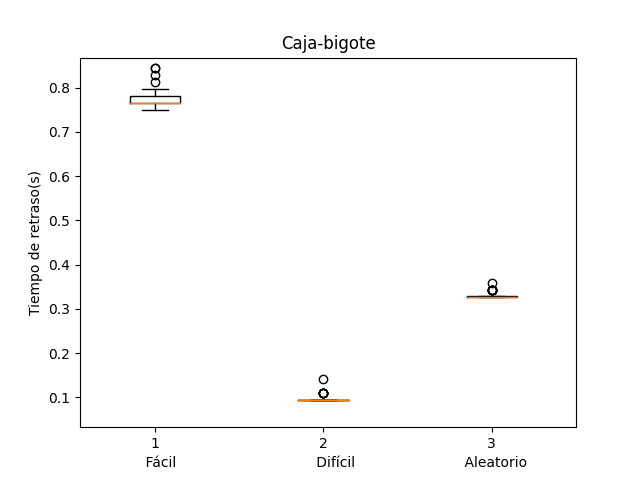
\includegraphics[scale=.6]{CB_1núcleos.png}
  \label{f1}
\end{figure}
\begin{figure}[H]
  \centering      
  \caption{Diagrama caja-bigote para 2 núcleos}  
  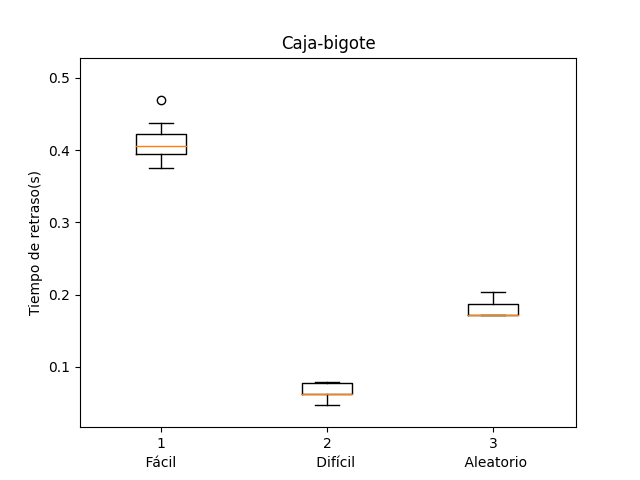
\includegraphics[scale=.6]{CB_2núcleos.png}
  \label{f2}
\end{figure}
\begin{figure}[H]
  \centering      
  \caption{Diagrama caja-bigote para 3 núcleos}  
  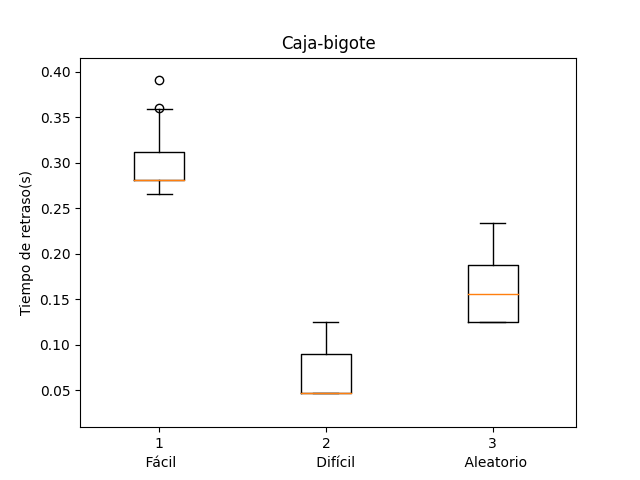
\includegraphics[scale=.6]{CB_3núcleos.png}
  \label{f3}
\end{figure}
\begin{figure}[H]
  \centering      
  \caption{Diagrama caja-bigote para 4 núcleos}  
  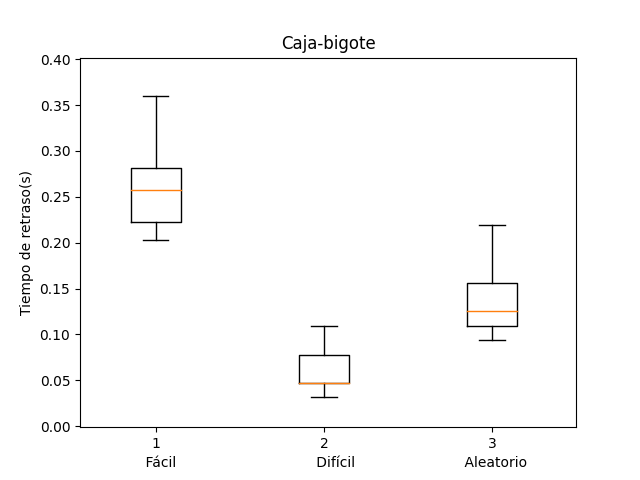
\includegraphics[scale=.6]{CB_4núcleos.png}
  \label{f4}
\end{figure}
\begin{figure}[H]
  \centering      
  \caption{Diagrama caja-bigote para 5 núcleos}  
  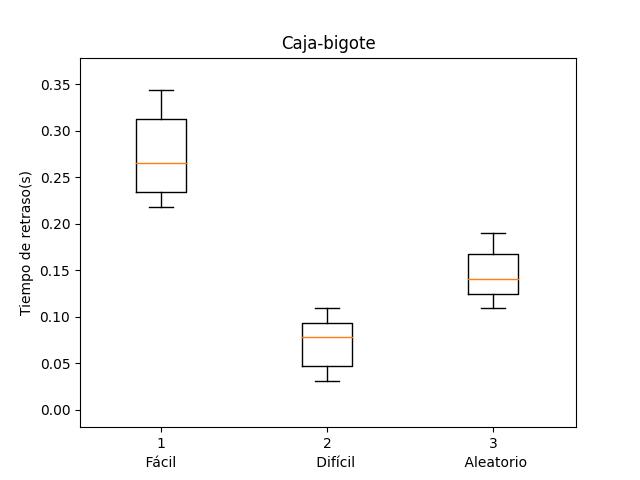
\includegraphics[scale=.6]{CB_5núcleos.png}
  \label{f5}
\end{figure}
\begin{figure}[H]
  \centering      
  \caption{Diagrama caja-bigote para 6 núcleos}  
  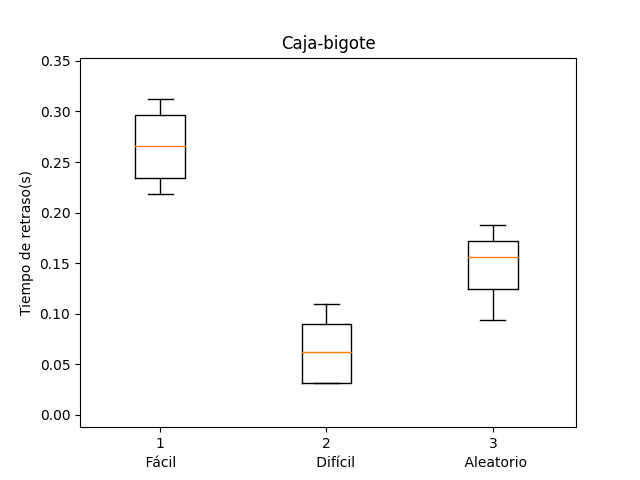
\includegraphics[scale=.6]{CB_6núcleos.png}
  \label{f6}
\end{figure}
\begin{figure}[H]
  \centering      
  \caption{Diagrama caja-bigote para 7 núcleos}  
  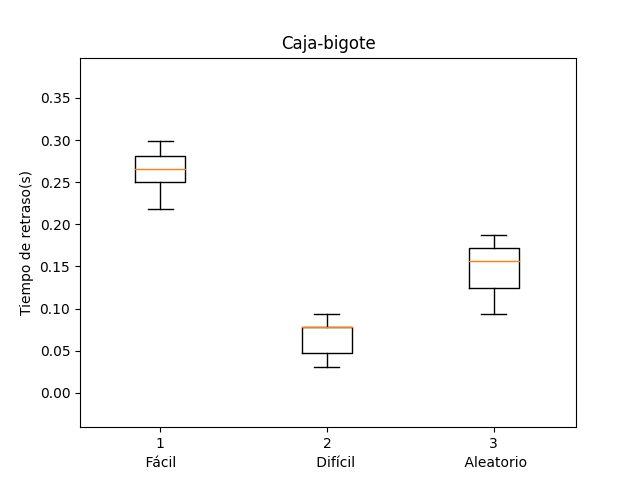
\includegraphics[scale=.6]{CB_7núcleos.png}
  \label{f7}
\end{figure}
\bigskip
\bigskip
Puede concluirse que la cantidad de núcleos asignados influye mucho en el tiempo de retraso en los trabajos debido a que si se reparten entre mas las tareas este tiempo reduce, dentro de este análisis si se va mas profundo al orden en que se asignan estas tareas se ve que el modo \textit{fácil} (no-primos a primos) es el que obtuvo el mayor tiempo de ejecución mientras que un orden \textit{difícil} (primos a no-primos) es ejecutado de manera mas rápida sin tanto tiempo de retraso, visto en la Figura \ref{f7} que la media de datos en difícil no sobrepasa .265 (s) para su mayor numero de núcleos trabajando.
 \bigskip
  \bigskip


\bibliography{refere}
\bibliographystyle{plainnat}




\end{document}
